\chapter{Projektplan}

Unseren Projektplan haben wir in zwei Phasen entwickelt, zu beginn eine Grobplanung und nach der endgültigen Ideenfindung und mit den erarbeiteten Use Cases konnten wir mit der Feinplanung beginnen. 

\begin{figure}[H]
	\centering
	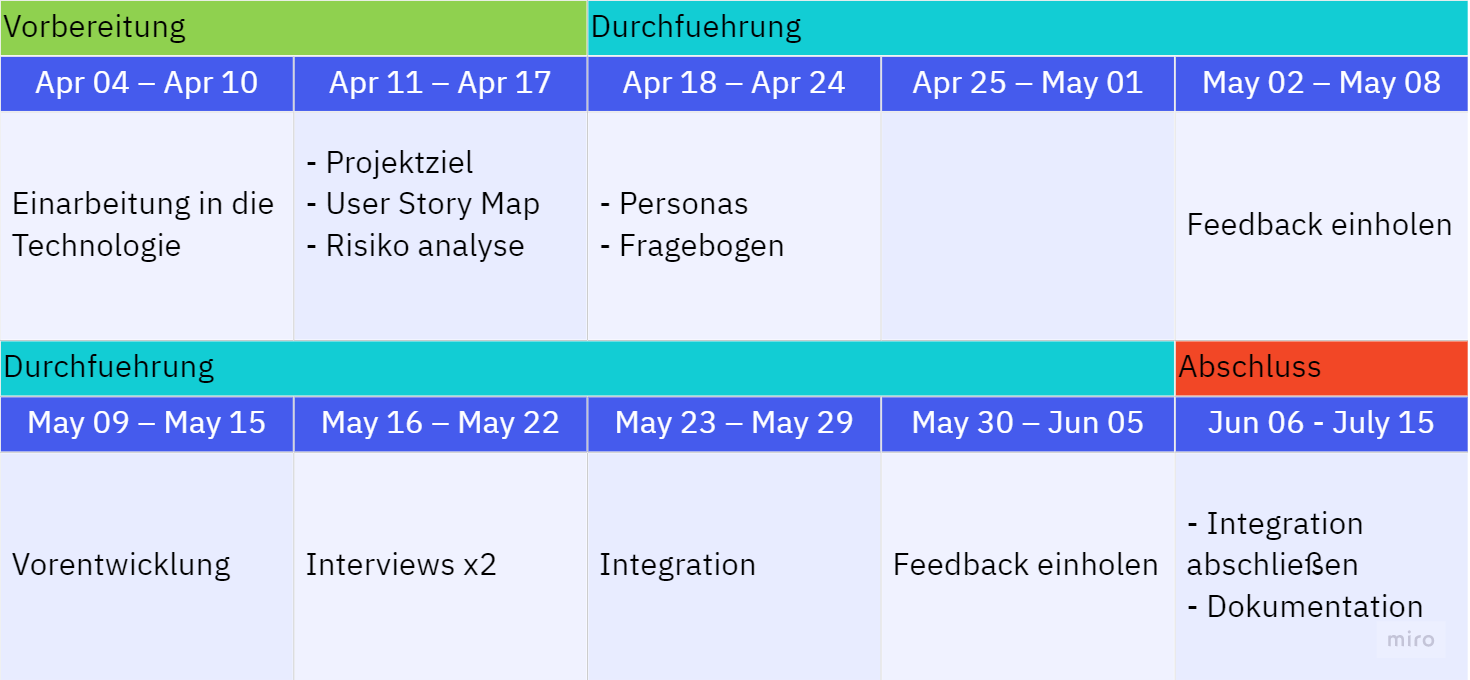
\includegraphics[width=0.95\textwidth]{coarse-plan}
    \caption{Grobplanung der Gruppe DEV-2\cite{coarsePlan2022}}
	\label{fig:coarse-plan}
\end{figure}

Aus den Use Cases hat sich folgende Feinplanung ergeben:



\begin{landscape}
    \begin{figure}[H]
        \centering
        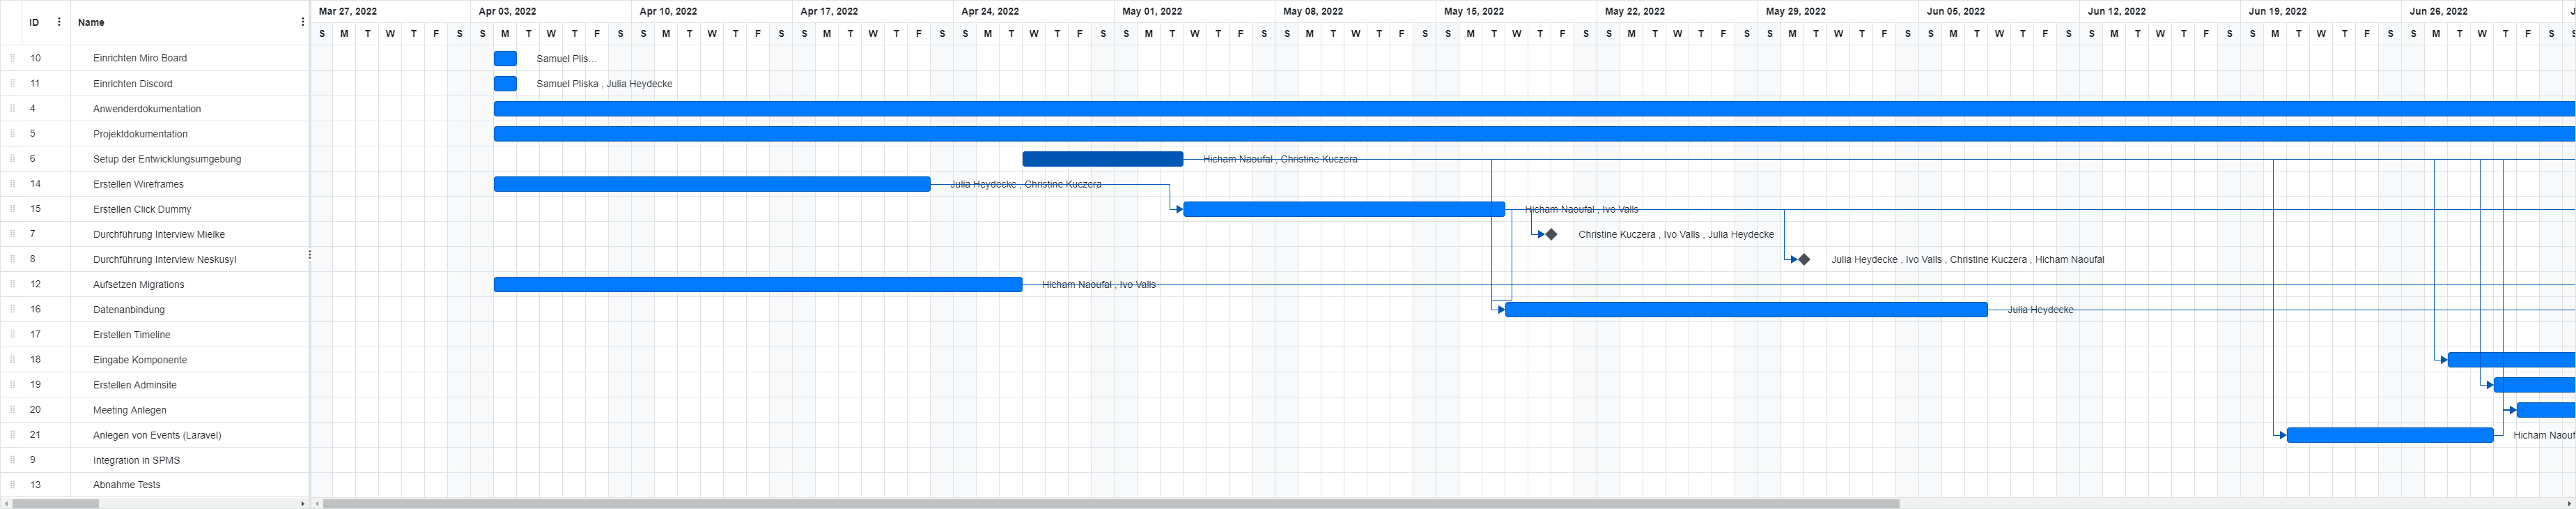
\includegraphics[width=23.5cm]{gantt}
        \caption{Feinplanung der Gruppe DEV-2\cite{finePlan2022}}
        \label{fig:fine-plan}
    \end{figure}
\end{landscape}